\section{Theoretischer Hintergrund}
\subsection{\ac{EDA}}
\subsubsection*{Fragen an diesen Abschnitt}
\begin{itemize}
    \item Was ist \ac{EDA}?
    \item Was ist ein Event?
    \item Warum ist \ac{EDA} relevant?
\end{itemize}
\subsubsection*{Ereignisorientierung als Architekturansatz}
Zuerst einmal handelt es sich bei \ac{EDA}\footnote{Da sich bis jetzt keine allgemeingültige deutsche Übersetzung der Fachterminologie durchgesetzt hat, sollen in dieser Arbeit die englischen Begrifflichkeiten verwendet werden.} um ein Konzept der Prozessmodellierung. Im Gegensatz zur gewöhnlichen Ablauf-orientierten Modellierung werden die Prozesse nicht als aufeinanderfolgende Schritte, sondern als Reaktionen auf Zustände konzeptioniert. Daraus resultiert, dass nicht mehr die prozedurale Abhandlung von Arbeitsschritten die zentrale Aufgabe in der Anwendungssystem-Entwicklung darstellt, sondern die Reaktion auf Ereignisse. Im Mittelpunkt von Architekturentscheidungen steht die Frage: "Was passiert, wenn dieses Ereignis eintritt?" und nicht mehr: "Welche Schritte müssen zur Erfüllung dieser Anforderung gegangen werden?". Was daraus resultiert, ist eine Architektur, die schon mit Beginn der Konzeption wesentlich agiler und robuster ist, da von Anfang an mit der Annahme gearbeitet wird, dass prinzipiell zu jedem Zeitpunkt jedes Ereignis eintreten kann.\footcite[Vgl.][S.30]{EDA2010}
Ein Definitionsversuch für \ac{EDA} könnte also wie folgt lauten: Event-Driven Archtitecture bezeichnet einen Modellierungsansatz für ein verteiltes, asynchrones System, das verschiedene Komponenten durch eine zentrale Verarbeitung von Events verbindet.\footcite[Vgl.][S. 248]{CLOUD2021}
\subsubsection*{Technische Grundkonzepte der \ac{EDA}}
\begin{figure}[H]
  \centering
	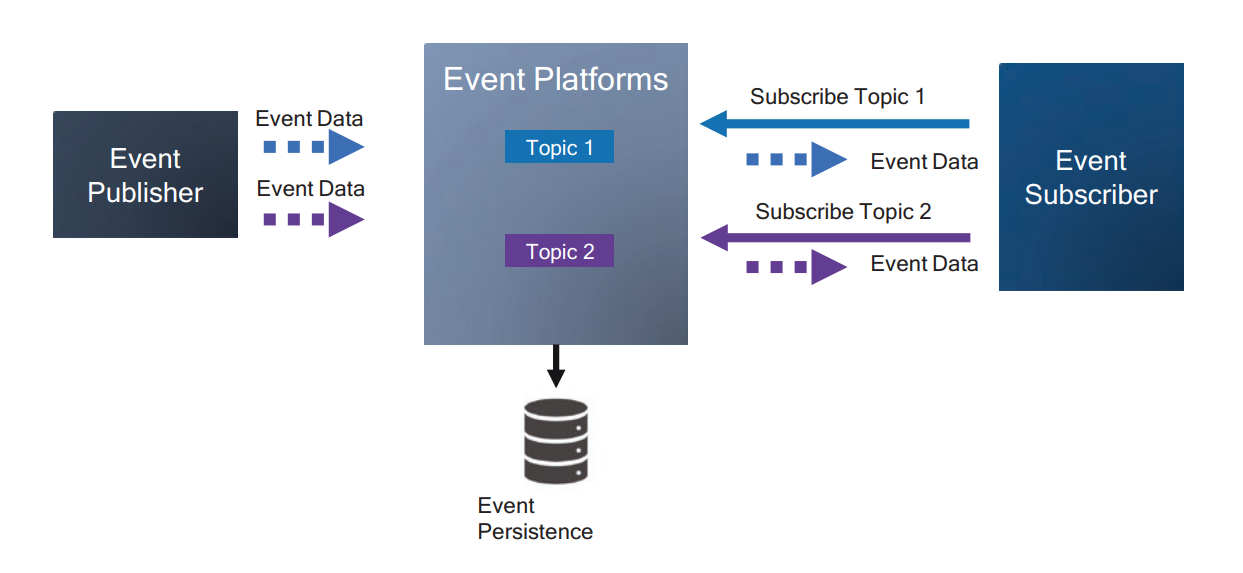
\includegraphics[width=0.8\textwidth]{Graphik EDA.png}
   \caption[Komponenten der \ac{EDA}]{Komponenten der \ac{EDA}\footnotemark}
\end{figure}
\footnotetext{\cite[][S. 249]{CLOUD2021}}
Die wichtigste Komponente eines durch \ac{EDA} modellierten Systems ist die zentrale Plattform zur Verarbeitung der Ereignisse in der Mitte der Architektur. Sie stellt die Infrastruktur bereit, um Events anzunehmen und diese weiterzugeben. Um einen Mehrwert aus dem System zu ziehen, muss sie darüber hinaus in der Lage sein, einen Kontext um Events herzustellen, d.h. sie in Verbindung mit anderen Ereignissen zu setzten, Ereignisse auf höheren Abstraktionsebenen zu erstellen und Ereignisse gegebenenfalls zu konsolidieren. Man spricht bei diesem Prozess von 
\ac{CEP}.\\
Weitere Komponenten des \ac{EDA} sind Publisher und Subscriber. \footnote{Für diese Komponenten finden sich in der Fachliteratur verschiedene Bezeichnungen. Außer Publisher und Subscriber findet man noch Producer und Receiver oder Producer und Listener.} Sie sind explizit von außen an das System herangeschaltet, d.h. sie haben keine Kenntnis voneinander und können auch auf völlig unterschiedlichen Plattformen basieren. Das bringt den Vorteil, dass ein durch \ac{EDA} modelliertes System inhärent modular aufgebaut ist und so zum einen weniger anfällig für Totalausfälle ist, da die Komponenten unabhängig sind, und zum anderen prädestiniert für Integrationsvorhaben ist.
Zu diesen grundlegenden Komponenten können im Zuge des \ac{CEP} noch einige weitere Konzepte hinzukommen. Die Abbildung zeigt beispielsweise eine Datenbank auf der Ereignisse persistent abgelegt werden können und die Einteilung von Ereignissen in Klassen, sogenannte Topics, die die Handhabung von verschiedenen Ereignisarten über ein System ermöglichen.
\subsubsection*{Ereignisse}
Zu klären bleibt die grundlegende Frage, was nun ein Ereignis ist. Die heute gängige Definition eines Ereignis im Kontext von \ac*{EDA} ist, dass ein Ereignis eine "signifikante Änderung des Zustands" ist.\footcite[Vgl.][S. 4]{EDA2006}


\subsection{RESTful \ac{API}}
\subsection{Technologie im Anwendungsbeispiel}
\subsection{Forschungsmethodik}
\subsection{Zusammenfassung des theoretischen Teils}



 
